\section{Implementation}
\label{sec:implementation}

\subsection{API Requirements and Design Goals}
\label{subsub:api-requirements-goals}

\paragraph{Orthogonality}
Most importantly though, the property  of orthogonality 
as defined by Eric S. Raymond in \textit{The Art of Unix
Programming} \cite{raymond2003compactness} has to be fulfilled for the visualization code with regards to the algorithm implementation's code, i.e. it should not change its behavior or state.

\paragraph{Declarativity} One of the main goals of this framework is to minimize 
the amount of code or configuration that has to be added to exisiting algorithms' implementations in order to make use of the visualization for its intended purpose in exploration or debugging. The visualization should therefore be specified as declaratively as 
possible, with the user specifying \textit{only} the relevant parameters–while minimizing the amount of required boilerplate code.

This allows for many side-effects like reusability, mainta

\paragraph{Separation of Concerns}
With the separation of the complex algorithm and user interface/visualization logic in mind is to keep the amount code required to create new visualizations as minimal as possible. 
Thus, we organize their architecture in a client-server 
relationship, whereby the client specifies the join 
problem parameters and configuration and the server can
generate a client-interpretable output to work with.

The advantages of this approach are multifold:
\begin{itemize}
    \item The server part and UI part respectively can be
          updated or even completely exchanged without 
          changing the other
    \item More complex join ordering algorithms can be 
          performed on a (more powerful) server
    \item The above allow us to run the application 
          within a web application without sacrificing 
          the performance by limiting ourselves with a 
          slow, interpreting JavaScript engine, but being 
          able to run compiled and thus more optimized and therefore faster 
          code
    \item (Allows us to formally specify interfaces between
          client and server) (Abbildung malen)
\end{itemize}

\paragraph{Flexibility}
The visualization tools should be abstract enough that it is not catered towards a specific algorithm, but can used to visualize a wide range of algorithms, especially ones it has not been explicitly programmed for.  

Since there is a large number of data structures an algorithm can use for its implementation we limit ourselves to procedures involving a query graph with information about its number of relations, the query graph type as specified in \ref{subsub:query-types}, and its cardinalities and selectivities.
This limitation is necessary to enfore a manageable scope for creating a minimum viable product.

More pragmatically, this means that the algorithm has to 
conform to the \texttt{Visualizable} Go type we define as 
follows:

\begin{figure}[H]
    \begin{minted}{go}
type Visualizable func(QG QueryGraph, JTC JoinTreeCreator) *Tree
    \end{minted}
    \caption{\texttt{Visualizable} type conformance requirement}
    \centering
\label{fig:visalizable}
\end{figure}

\begin{example}
This way, a Go function \texttt{DPccp} that conforms to this type can be instructed to produce the output  log necessary for the visualization by simply calling 

\begin{minted}{go}
Visualize(DPccp, QG, JTC)
\end{minted}
instead of the algorithm itself. The \texttt{visualize} function then automatically sets the appropriate flags to enable visualization output and can allow the algorithm to run without the visualization code and thus no (significant) runtime or memory overhead.

\end{example}

\paragraph{High signal-to-noise ratio} 
In our implementation we are using code folding, enabled
through the orthogonality property as mentioned in 
section \ref{subsub:api-requirements-goals}. This allows
us to completely show or hide the visualization code 
when required. Thus, we can achieve an inobtrusive
debugging tool that can be written alongisde an 
algorithm's implementation code and doesn't decrease
its signal-to-noise ratio.

\paragraph{Query Graph Planarity}
The visualized query graph should be drawn in a way that no edges are overlapping. This is possible when the query graph is \textit{planar} \cite{trudeau2013introduction}.


\subsection{Architecture}

The following figure \ref{fig:sequence-diagram} illustrates a sequence diagram for the client-server architecture used for this project. At first, we retrieve all avaialable algorithms, denoted by $A$, from the server. This is used to asynchronously generate the available options in the algorithm selection picker. Retrieving the algorithms from the server has the advantage that new algorithm visualizations can be added server-side without changing, re-installing or re-deploying any client code.

Next up, the user can select all the parameters for the visualization. The first parameter is the algorithm $a \in A$ to be visualized. Moreover, the query graph type $qg \in {\text{\{``chain'', ``star'', ``cycle'', ``tree'', ``moerkotte''\}}}$ can be specified. Contrary to the algorithm, the query type is not fetched from the server as the client implementation explicitly has to know the available query graphs at build time, since they are used for calculating the position of different query graph nodes as detailed in section \ref{subsub:query-graphs}. 

Furthermore, the number of relations in the query graph $n$ has to be specified, whereby $n \in [3,10]$. The upper boundary for $n$ is set to 10 to prevent calculations that are too complex and might be set even lower for algorithms other than \texttt{DPccp}, where the execution time and produced output is even larger.

Depending on the previously selected parameters the algorithm's steps are fetched upon clicking the ``Recalculate'' button. This will trigger another HTTP server request that transmits the algorithm (:a), number of relations (:r) and graph type (:g) as path parameters.

As the server receives this request, it calls the corresponding algorithm by using the \texttt{Visualize()} function specified in section TODO: ref. This produces a JSON response containing the query graph $QG$ with information about cardinalities, selectivities, and neighbors, as well as the algorithm's generated visualization steps $S$.

Upon receiving this response, the client renders the query graph including labels for cardinalities and selectivities, and edges for connected query graph nodes. Moreover, the algorithm's steps are rendered in a hierarchical table.

As the rendering completes, the number of total steps |S| is calculated and the user is presented with two buttons to move to either the next or the previous step. After doing so, the user interface, including the query graph and the variable table, are rerendered accordingly.

\begin{figure}[H]
    \centering
    \begin{sequencediagram}
        \def\unitfactor{0.9}
        \newthread{A}{Client (GUI)}{}
        \newinst[8]{B}{Server}{}
        \begin{call}{A}{Render UI}{A}{}
        \end{call}
        \begin{call}{A}{GET /api/algorithms}{B}{available algorithms $A$}
        \end{call}
        \begin{call}{A}{Render algorithm picker}{A}{}
        \end{call}
        \begin{sdblock}{loop}{}
            \begin{call}{A}{Choice of algorithm, query graph type, number of relations}{A}{}
            \end{call}
            \begin{call}{A}{GET /api/algorithm/:a/relations/:r/graphType/:g}{B}{query graph $QG$, algorithm steps $S$}
            \end{call}
            \begin{call}{A}{Render query graph, algorithm steps}{A}{}
            \end{call}
            \begin{sdblock}{loop}{}
                \begin{call}{A}{User moves to next or previous step}{A}{Rerender UI}
                \end{call}
            \end{sdblock}
        \end{sdblock}
    \end{sequencediagram}
    \caption{UML sequence diagram of the client-server communication}
    \label{fig:sequence-diagram}
\end{figure}


\subsection{Choice of Technology}

For the implementation of both client and server code we
want to maximize

\begin{enumerate}[label={(\roman*)}]
    \item \label{itm:accessibility} \textbf{Accessibility}, a minimal amount of effort required to access the application
    \item \label{itm:maintainability} \textbf{Maintainability}, a high degree of technological similarities with related projects 
    \item \label{itm:testedness} \textbf{Tried-and-testedness}, a large user base and well-received reference applications
\end{enumerate}

In order to maximize \ref{itm:accessibility} we create an application that runs in a web browser and doesn't need any user-initiated installation or update procedures.
With the 2017 released WebAssembly (Wasm)\footnote{\url{https://webassembly.org}} portable byte-code standard still being in its infancy at around 90\% browser support\footnote{\url{https://caniuse.com/wasm}} and being recommended by the World Wide Web Consortium not until December 5th 2019\footnote{\url{https://www.w3.org/TR/wasm-core-1/}}, this leaves us with JavaScript as the only viable language for the client-side code. 

Additionally, in order to modularize the user interface and adding the ability to import existing user interface components, we use \texttt{React.js}\footnote{\url{https://reactjs.org}}, as of writing this thesis the most popular JavaScript library for building user interfaces.
%\footnote{Ranked by number of stars on \url{https://github.com/search?l=JavaScript&o=desc&q=language%3AJavaScript&s=stars&type=Repositories}}.
% search?l=Go&o=desc&q=http&s=stars&type=Repositories

For the server code and algorithm implementations we use the Go programming language and \texttt{gin-gonic}\footnote{\url{https://github.com/gin-gonic/gin}}, which at the time of writing this thesis is the most-starred HTTP framework on GitHub\footnote{\url{https://github.com/}}.

%Thus, we resort to modern, but well-adopted languages and libraries.
%The software should be built with technologies that prepare well for continued development and maintenance.

\subsection{Tooling}

\subsubsection{Join Problem Generator}
We represent the join problems in a JSON format as defined in section \ref{subsub:join-problem-data-structure}. 
Some JSON files are taken from the supplementary material to the ``IE 630 Query Optimization'' course exercises at the University of Mannheim\footnote{\url{https://www.wim.uni-mannheim.de/moerkotte/teaching/courses/query-optimization/}}
, which contains examples for join problems with a query type $QT \in $ \{Chain, Clique, Cycle, Star\} and a number of relations $n \in [2,10]$.

Additionally, we create a join problem generator for complete binary trees with a degree $k$ and a number of relations $n$.

Since selectivities are symmetrical, they are stored once and once only in the JSON. This means, if an edge ($R_0, R_1$) in the query graph exists, we don't store ($R_1, R_0$) explicitly as well. However, we store the selectivities in a breadth-first manner starting from $R_0$, i.e. the edge always points from the relation with the smaller index to the larger one. More formally, we can say that the following implication holds:

\begin{equation}
    \forall (R_i, R_j) \in E \implies i < j
\label{eq:bfs-implication}
\end{equation}

\setlength{\belowdisplayskip}{10pt}
\setlength{\belowdisplayshortskip}{50pt}
\setlength{\abovedisplayskip}{10pt}
\setlength{\abovedisplayshortskip}{10pt}

\paragraph{Complete Binary Tree}
\subparagraph{Selectivities}
Since implication \ref{eq:bfs-implication} holds, we only need to calculate selectivities for nodes which have children.
Thus, first of all, we calculate the number of vertices with children $n_c$, i.e. the number of relation-pairs for which selectivity entries exist in the resulting JSON file.
In the case of complete $k$-ary trees, when enumerating the relations in a breadth-first manner, this number is given by 
\begin{equation}
    n_{c} = \#\{v \in V \vert \text{hasChildren}(v)\} = \lceil\frac{n}{k}\rceil
\end{equation}
Accordingly, we specify the set of vertices with children $V_c$, starting with index 0.
\begin{equation}
   V_c := \{v_i\}_{i=0}^{n_{c}-1}
\end{equation} 

\begin{note}
Let $I$ be the index set for all relations
\begin{equation}
    I = \{0,\ldots,n-1\}
\end{equation}
Then, since our $k$-ary tree is complete and breadth-first, we can infer that if a node at index $i$ does not have children, any node at a larger index $j$ doesn't either. Likewise, any node with an index $i < n_c$ does have children. 

\begin{equation}
    \forall i,j \in I, i < j \colon v_i \notin V_c \implies v_j \notin V_c
\end{equation}
\begin{equation}
    \forall i < n_c \colon \exists v_i \in V_c
\end{equation}

This is why it suffices to consider nodes with index $i < n_c$ when generating selectivity entries.
\end{note}

Furthermore, we need to determine the level $l(v_i)$ of each node $v_i$ in the tree. For its respective index $i$, this is given by
\begin{equation}
    l_i = l(v_i) = log_k(i+1)
\end{equation}

Next up, we then define the set of vertices in the levels below $l_i$, denoted $V_{l_{i<j}}$, as follows:
\begin{equation}
    V_{l_{j<i}} := \{v_j \in V \vert l(v_j) < l(v_i) \}
\end{equation}

Now, we need the cardinality of this set, defined as $n_{j<i}$ to get the number of nodes on all level smaller than $l_i$. This can be efficiently calculated using the following equation:
\begin{equation}
     n_{j<i} := \vert V_{l_{j<i}}\vert = 2^{l(v_i) + 1} - 1
\end{equation}

This allows us to calculate the number of children for each level $l(v_i)$.
\begin{equation}
    \hat{l}_i = \min(2^{l(v_i) + 1}, n - n_{j<i})
\end{equation}

\begin{note}
Note that $l(v_i)$ is not necessarily equal to the width of the level in a full $k$-ary tree, which is given by $2^{l(v_i) + 1}$, since some leaf nodes could be missing in the bottom level of the tree.
\end{note}

Furthermore, we calculate the ``column'' $c_i$ of $v_i$, given by
\begin{equation}
    c_i = i - 2^{l(v_i)} + 1
\end{equation}

This lets us calculate the number of children $\hat{n}_i$ for a node at index $i$:
\begin{equation}
    \hat{n}_i = \min(k, \hat{l} - c_i * k)
\end{equation}

\begin{note}
    This $\hat{n}_i$ is equal to $k$ for most internal nodes in a sufficiently large tree. However, if $log_k(n) \notin \mathbb{N}$ there could be an internal node with $\hat{n}_i < k$, i.e. not all possible leaf nodes for the last node with childrens are filled.
\end{note}

Now we can define the neighbors of $v_i$ as
\begin{equation}
    \mathbb{N}_i = \{ x_{i, j} \}_{j=0}^{\hat{n}_i - 1} 
\end{equation}

We also calculate the lowest index of the node's neighbors $j_{min\mathbb{N}_i}$. (TODO: Not entirely sure about this notation).
\begin{equation}
    j_{min\mathbb{N}_i} = ik + 1
\end{equation}

For each neighbor $x_{i, j} \in \mathbb{N}_i$ we then calculate the offset for its $j$ index.
\begin{equation}
    \tau_{i,j} = j\mod{k}
\end{equation}

The current index of the neighbor is thus given by
\begin{equation}
    \sigma_{i,j} = j_{min\mathbb{N}_i} + \tau_{i,j}
\end{equation}

Finally, we can set all $x_{i, j} \in \mathbb{N}_i$ as $\sigma{i,j}$
\begin{equation}
    x_{i, j} = \sigma_{i,j}
\end{equation}

Let us now define the set of all neighbors $\mathbb{N}$ for all indices $i < n$:
\begin{equation}
    \mathbb{N} = \{\mathbb{N}_i\}_{i=0}^{n-1}
\end{equation}

We can now set a selectivity for each $(x_i,j) \in \mathbb{N}_i \in \mathbb{N}$, where the selectivity $s_{i,j}$ is a random varialbe following a uniform distribution over the set $\mathbb{R} \cap [0,1]$.

A Go implementation example of the symmetrical neighbor calculation is illustrated in algorithm \ref{alg:symNeighbors}. The assignment of selectivities to these entries is trivial and thus not illustrated here, but can be found in the supplementary code.

\begin{note}
The variable names in algorithm \ref{alg:symNeighbors} correspond to the names used in the previously used mathematical definitions. In the supplementary code to this thesis longer, more descriptive variable names are used.
\end{note}

%TODO: Replace \texttt{log2_{64}} with \texttt{math.Log}

\begin{algorithm}[H]
\begin{minted}{go}
symNeighborEntry := func(i uint, n_c uint) string {
    l_i := uint(log2_64(uint64(i + 1)))
    n_j_leq_i := uint(1<<(l_i+1) - 1)
    l_hat_i := min(1<<(l_i+1), n-n_j_leq_i)
    c_i := i - 1<<(l_i) + 1
    n_hat_i := min(k, l_hat_i-c_i*k)

    N := make([]string, n_c)
    j_minN_i := i*k + 1
    for j := range N {
        tau_ij := uint(j) % k
        sigma_ij := j_minN_i + tau_ij
        s := strconv.FormatUint(uint64(sigma_ij), 10)
        N[j] = s
    }
    return strings.Join(N, ",")
}
symNeighbors := func() map[uint]string {
    dict := map[uint]string{}
    n_c := math.Floor(float64(n) / float64(k))
    for i := uint(0); float64(i) < n_c; i++ {
        dict[i] = symNeighborEntry(i, n)
    }
    return dict
}
neighbors := symNeighbors()
\end{minted}
\caption[Go implementation to calculate symmetrical neighbors]{Go implementation to calculate symmetrical neighbors. \texttt{k} is the degree of the tree and \texttt{n} the number of relations. Both must be set before using them in the above lambda expressions (Go function literals).}
\label{alg:symNeighbors}
\end{algorithm}

\subparagraph{Neighbors}
The set of neighbors does not make use of the symmetry of selectivities and thus stores all neighbors for each relation explicitly. Thus, we append the parent node $\rho_i$ to the set of neighbors $\mathbb{N}$ calculated for the selectivity generation. This assignment is trivial and thus the algorithm is not provided here.

% We then join all $$
% Joining x_{i, j} into array for each i
\subparagraph{Relations}
Specifying the relations $R$ is trivial. 

\begin{equation}
R := \{R_i\}_{i=0}^{n-1}
\end{equation}
where the cardinality $c_{r_i}$ of each relation $r_i$ is a random variable following uniform distribution over the set $\mathbb{R} \cap [0,10000]$.

Likewise, the creation of the Go \texttt{relations} slice is trivial and therefore we don't illustrate the algorithm here.

\subsection{Data Structures}
\label{sub:data-structures}

\subsubsection{Join Ordering}
In order to parse and represent a join problem from a JSON file we use the already existing data structures \texttt{JSONRelation} and \texttt{JSONJoinProblem} from \texttt{joinProblemParser.go}. Both are implicitly marshalled and unmarshalled when converted from or to JSON because of the built-in JSON encoding and decoding for custom data structures using the Go standard library's \texttt{encoding/json} package\footnote{\url{https://golang.org/pkg/encoding/json/}}. However we add \texttt{struct} tags to explicitly set the corresponding JSON keys.
\vspace{0.6cm}

\begin{code}
\begin{minted}{go}
type JSONRelation struct {
    Cardinality float64 `json:"cardinality"`
    Name        string  `json:"name"`
    ProblemID   uint    `json:"problemID"`
    RelationID  uint    `json:"relationID"`
}
\end{minted}
\caption{\texttt{JSONRelation} type}
\end{code}
\vspace{0.6cm}

\begin{code}
\begin{minted}{go}
type JSONJoinProblem struct {
    ProblemID         uint               `json:"problemID"`
    Neighbors         map[uint]string    `json:"neighbors"`
    NumberOfRelations uint               `json:"numberOfRelations"`
    Relations         []JSONRelation     `json:"relations"`
    Selectivities     map[string]float64 `json:"selectivities"`
}
\end{minted}
\caption{\texttt{JSONJoinProblem} type}
\end{code}
\vspace{0.8cm}

We'll take the \texttt{QueryGraph} \texttt{struct} from \texttt{infra.go} and add a \texttt{map} to a \texttt{uint} slice of neighbors for each relation, which itself is represented as a \texttt{uint} bitvector and used as the map's key.

\begin{code}
\begin{minted}{go}
type QueryGraph struct {
	R []uint           `json:"relationCardinalities"`
	S map[uint]float64 `json:"selectivities"`
	N map[uint][]uint  `json:"neighbors"` // Added neighbor map
}
\end{minted}
\caption{\texttt{QueryGraph} type}
\end{code}
\vspace{0.8cm}



Also, we introduce a struct for representing csg-cmp-pairs.
\begin{code}
\begin{minted}{go}
type CsgCmpPair struct {
    S1 uint
    S2 uint
}
\end{minted}
\caption{\texttt{CsgCmpPair} type}
\label{datastructure:csg-cmp-pair}
\end{code}

\vspace{0.8cm}

\subsubsection{Visualization}

For the visualization we define some data structures used to declaratively specify algorithms, their visualization routines and their atomic components, such as visualization steps and the subroutine's configured observed relations. 

\paragraph{Algorithm}

First, we specify an \texttt{Algorithm} type that can be returned to the client when requesting the list of algorithms which can be visualized. Each algorithm contains a \texttt{Label} string describing the algorithm, e.g. ``DPccp'' as well as a \texttt{Value} string giving the algorithm's identifier for server requests. This \texttt{Value} string is by convention a camel-cased name of the algorithm starting with a lower-case character, whereas the \texttt{Label} can also contain special or whitespace characters. This differentiation is made to allow human-readable algorithm names as well as URL-encodable identifiers for the API's path parameter.

\begin{code}
\begin{minted}{go}   
type Algorithm struct {
    Label string `json:"label"`
    Value string `json:"value"`
}
\end{minted}
\caption{\texttt{Algorithm} type}
\end{code}
\vspace{0.8cm}

\paragraph{Variable Table}

We want to keep track of a set of user-defined relation variables to aid understanding the algorithm's state's history. For this purpose, we first introduce the \texttt{ObservedRelation} type that can be used to specify which sets of relations should be observed. It contains an \texttt{Identifier} string that corresponds to the variable's name, as well as a \texttt{Color} field, which allows to visually distinguish different variables. This is specified using a \texttt{color.RGBA} struct from the \texttt{image/color} package, which can be found in Go's standard library.

\begin{code}
\begin{minted}{go}
type ObservedRelation struct {
    Identifier string     `json:"identifier"`
    Color      color.RGBA `json:"color"`
}
\end{minted}
\caption{\texttt{ObservedRelation} type}
\end{code}
\vspace{0.8cm}

Furthermore, we introduce a \texttt{VariableTableEntry} type that can be specified individually for each observed relation, in each atomic visualization step. In our application, this entry is a \texttt{uint} slice depicting the current variable's set of relations in bitvector representation.

\begin{code}
\begin{minted}{go}
type VariableTableEntry []uint
\end{minted}
\caption{\texttt{VariableTableEntry} type}
\end{code}
\vspace{0.8cm}

TODO: Rename in code
These variable table entries are stored in a \texttt{VariableTableRow} map. A string identifying the relation that corresponds to the \texttt{Identifier} in the \texttt{ObservedRelation} as the key of the map.

\begin{code}
\begin{minted}{go}
type VariableTableRow map[string]VariableTableEntry
\end{minted}
\caption{\texttt{VariableTableRow} type}
\end{code}
\vspace{0.8cm}

\paragraph{GraphState}

The state of the query graph drawn in the user interface must be represented in order to unambigiously specify its configuration. We want to be able to give each node in the graph a color that corresponds to the \texttt{Color} field of the \texttt{ObservedRelation}. Hence, we first define a \texttt{NodeColor} type storing the \texttt{Index} of the relation, as well as the respective \texttt{Color}.

\begin{code}
\begin{minted}{go}
type NodeColor struct {
    NodeIndex uint       `json:"nodeIndex"`
    Color     color.RGBA `json:"color"`
}
\end{minted}
\caption{\texttt{NodeColor} type}
\end{code}
\vspace{0.8cm}

The graph state is thus a slice containing all node colors. Since we explicitly assign a color to each node in every visualization step, the length of the slice is therefore equal to the number of relations $n$ in the graph.

\begin{code}
\begin{minted}{go}
type GraphState struct {
    NodeColors []NodeColor `json:"nodeColors"`
}
\end{minted}
\caption{\texttt{GraphState} type}
\end{code}
\vspace{0.8cm}

\paragraph{Steps and Routines}

Finally, the data structures defined beforehand can be used to construct higher-level constructs such as the \textit{atomic} visualization step, represented as a \texttt{VisualizationStep} type. This type contains the \texttt{GraphState} for the current step, as well as the variables stored as a \texttt{VariableTableRow}. In order to identify a step in equivalence checks, we also assign a \texttt{UUID}, which is generated using Google's own \texttt{github.com/google/uuid}\footnote{\url{https://github.com/google/uuid}} package. This UUID is a 128 bit UUID based on RFC4122\footnote{\url{https://tools.ietf.org/html/rfc4122}}, which can be easily converted to a \texttt{string} using the \texttt{uuid.New().String()} function. This \texttt{UUID} is necessary as the reference to the exact instance of a struct is lost when marshalling it into JSON.

\begin{code}
\begin{minted}{go}
type VisualizationStep struct {
    GraphState GraphState       `json:"graphState"`
    Variables  VariableTableRow `json:"variables"`
    UUID       string           `json:"uuid"`
}
\end{minted}
\caption{\texttt{VisualizationStep} type}
\end{code}
\vspace{0.8cm}

Finally, we have defined all the types necessary to define a high-level \texttt{VisualizationRoutine}. This routine contains a \texttt{Name} field to describe its corresponding algorithm, e.g. ``EnumerateCsg'', as well as fields to store an \texttt{ObservedRelation} slice to specify the sets of relations that should be kept track of for this routine. Furthermore, we store a slice of all the routines steps. This \texttt{Steps} slice is genericly implemented using a pointer to Go's \texttt{interface{}} type, as it can be filled with either an atomic \texttt{VisualizationStep} or another \texttt{VisualizationRoutine}. This allows for subroutines or even recursive calls of other subroutines and creates a hierarchical structure of all steps in the visualization's JSON representation. 

\begin{code}
\begin{minted}{go}
type VisualizationRoutine struct {
    Name              string             `json:"name"`
    ObservedRelations []ObservedRelation `json:"observedRelations"`
    Steps             []*interface{}     `json:"steps"`
}
\end{minted}
\caption{\texttt{VisualizationRoutine} type}
\end{code}
\label{datastructure:visualization-routine}
\vspace{0.8cm}

This \texttt{VisualizationRoutine} is transferred as a top-level object when making a server request and thus we don't need to specify any more data structures.

\subsection{Server Implementation}

\subsubsection{Utility Functions}

In order to provide a starting point for the algorithm implementation, we use a modified and extended version of the \url{infra.go} and \url{joinproblemparser.go} file provided for the exercises in the Query Optimization (CS50x) course \texttt{} at the Chair of Practical Computer Science III at the University of Mannheim.

Modifications include:
\paragraph{Simplification of \texttt{SetMinus}}
We simplify the implementation for the \texttt{SetMinus} operation by omitting the use of a temporary helper variable for the result calculation. This is equivalent as it produces exactly the same assembly output as the old, commented-out code\footnote{using amd64 gc 1.15 compiler, compiled on \url{https://godbolt.org}}.

\begin{algorithm}
\begin{minted}{go}
func SetMinus(S1 uint, S2 uint, length uint) uint {
    mask := uint((1 << length) - 1)
    // temp := S1 & S2
    // temp = ^temp
    // temp &= mask
    // return S1 & temp
    return S1 & ^S2 & mask
}
\end{minted}
\caption{Go implementation of \texttt{SetMinus}}
\label{alg:implementation-setminus}
\end{algorithm}

\paragraph{Addition of \texttt{PowerSet}}
For the implementation of \texttt{DPccp} we need an additional function that returns not just the subsets of an (\texttt{unsigned int}) bit vector $S$ as does \texttt{Subsets}, but its power set excluding the empty set, $\mathcal P(S)\setminus\{\varnothing\}$.

\begin{algorithm}
\begin{minted}{go}
func PowerSet(S uint) []uint {
    subsets := Subsets(S)
    if len(subsets) == 1 && subsets[0] == S {
        return subsets
    }
    return append(subsets, S)
}
\end{minted}
\caption{Go implementation of \texttt{PowerSet}}
\label{alg:implementation-powerset}
\end{algorithm}

Furthermore, we add a function to calculate the minimum element of a \texttt{[]uint} slice, as well as a function to get the minimum set bit index for a (sub-)set of relations $S$, which makes use of the former.

\begin{algorithm}[H]
\begin{minted}{go}
func MinUintSlice(slice []uint) uint {
    if len(slice) == 0 {
        return uint(0)
    }
    min := slice[0]
    for _, value := range slice {
        if min > value {
            min = value
        }
    }
    return min
}

func MinUintSetBitIndex(S uint) uint {
	setIndexes := IdxsOfSetBits(S)
	minIndex := MinUintSlice(setIndexes)
	return minIndex
}
\end{minted}
\caption{Go implementation of \texttt{MinUintSlice} and \texttt{MinUintSetBitIndex}}
\label{alg:implementation-minuintslice}
\end{algorithm}
\vspace{0.5cm}

% We add some additional helper functions:
% \begin{minted}{go}   
% func contains(s []uint, e uint) bool {
%     for _, a := range s {
%         if a == e {
%             return true
%         }
%     }
%     return false
% }    
% \end{minted}

Moreover, we'll add a method to retrieve the neighborhood for a subset of relations $S$.

\begin{algorithm}[H]
\begin{minted}{go}
func Neighbors(QG QueryGraph, S uint) uint {
    indexes := IdxsOfSetBits(S)
    result := uint(0)
    for _, index := range indexes {
        for _, neighbor := range QG.N[index] {
            result = result | (1 << neighbor)
        }
    }
    n := uint(len(QG.R))
    return SetMinus(result, S, n)
}
\end{minted}
\caption{\texttt{Neighbors} function for a set of relations}
\end{algorithm}
\vspace{0.5cm}

\subsubsection{Visualization}

For the visualization we create a \texttt{visualization} package to handle all operations related to the visualization itself. 

Here, we keep track of an exported \texttt{VisualizationOn} Boolean variable to indicate whether the visualization code within the algorithm's implementation should be executed or not. Furthermore, we define two package-local variables:
\vspace{0.2cm}
\begin{minted}{go}
var routines = []*VisualizationRoutine{}
var stack = []*VisualizationRoutine{}
\end{minted}
\vspace{0.2cm}
Both variables are slices of pointers to the \texttt{VisualizationRoutine} type defined in figure \ref{datastructure:visualization-routine}. They both fulfill different purposes: the former keeps track of consecutively executed visualization routines, whereas the latter stores the  execution stack of the current routine, which allow for stacked or recursive routine calls. In order to enforce modularity, those variables cannot be changed directly, but tjhe exported functions to start new routines or add atomic visualization steps have to be used. All available functions will be discussed in the following.

First of all, we create a \texttt{visualize} function to change the execution context of a join ordering algorithm.
\begin{minted}{go}
func Visualize(visualization Visualizable, 
               QG QueryGraph, 
               JTC JoinTreeCreator) []*VisualizationRoutine
\end{minted}

This \texttt{visualize} function can be used to call a function that conforms to the \texttt{Visualizable} type as defined in \ref{fig:visalizable}, one example being our implementation of \texttt{DPccp}. This will automatically set the \texttt{VisualizationOn} Boolean to \texttt{true}, execute the algorithm, and set it back to its previous value after finishing the execution. Moreover, it will return all the emitted routines as a \texttt{*ViszalizationRoutine} slice and reset all local variables after execution.

\begin{example}
    An implementation of the \texttt{DPccp} algorithm defined through the following function
    \begin{minted}{go}
func DPccp(QG QueryGraph, JTC JoinTreeCreator) *Tree
    \end{minted}
    can be visualized by calling
    \begin{minted}{go}
Visualize(DPccp, QG, JTC)
    \end{minted}
    instead of directly calling
    \begin{minted}{go}
DPccp(QG, JTC)
    \end{minted}
\end{example}

\begin{note}
Notice that the function definition of \texttt{DPccp} doesn't have to be changed from its original implementation at all here. Thus, potenitially already existing calls to \texttt{DPccp} don't have to be modified.
\end{note}

Within the function implementation we can now use the exported visalization functions to start new routines and add new visualization steps. Before adding the first step, we have to call the following function at least once: 
\begin{minted}{go}
func StartVisualizationRoutine(routine *VisualizationRoutine)
\end{minted}

As the name implies, this function can be used to start a new visualization routine. This will add a new routine to the \texttt{routines} slice if the current call stack is empty or push it to the stack if there's already a function being executed. Notice that whether the function is introduced as a consecutive routine or added to the call stack is determined by the \texttt{visualization} package implicitly, for the convenience of the package's user. An example how this call stack could look like for \texttt{DPccp} at a certain point in its execution is shown in figure \ref{fig:execution-stack}, with the most recent subroutine pushed onto the top of the stack.

\begin{figure}[H]
\begin{tikzpicture}[stack/.style={rectangle split, rectangle split parts=#1,draw, anchor=center}]
    \node[stack=5]  {
        \nodepart{one}EnumerateCsgRec
        \nodepart{two}EnumerateCsgRec
        \nodepart{three}EnumerateCsgRec
        \nodepart{four}EnumerateCsg
        \nodepart{five}DPccp
    };
    \end{tikzpicture}
\caption{Sample excution stack for \texttt{DPccp}}
\label{fig:execution-stack}
\end{figure}

After starting a visualization routine we either start a new routine that is added onto the stack or add a visualization step using the following function, which takes a \texttt{QueryGraph} and a \texttt{VariableTable} as its parameters.

\begin{minted}{go}
func AddVisualizationStep(QG QueryGraph, relations VariableTable)
\end{minted}

The implementation of this function will automatically construct a new \texttt{GraphState} from information in the passed \texttt{VariableTable} by retrieving its respective color configuration. This makes sure the observed relations and their corresponding nodes in the query graph have the same color without the need to specify it separately or explicitly creating the \texttt{GraphState}. Furthermore, a \texttt{UUID} is assigned to the visualization step, which used for efficient equivalence checks in the client implementation.

\begin{fullwidth}[width=\textwidth + 0.5cm,leftmargin=-2.5cm]
\begin{algorithm}[H]
\begin{minted}{go}
func AddVisualizationStep(QG QueryGraph, relations VariableTable) {
    n := uint(len(QG.R))
    nodeColors := []NodeColor{}
    currentStackIndex := len(stack) - 1
    observedRelations := stack[currentStackIndex].ObservedRelations
    for i := n - 1; int(i-1) >= -1; i-- {
        for _, relation := range observedRelations {
            relationIndexes := relations[relation.Identifier]
            if contains(relationIndexes, i) {
                color := relation.Color
                nodeColor := NodeColor{NodeIndex: i, Color: color}
                nodeColors = append(nodeColors, nodeColor)
            }
        }
    }
    graphState := GraphState{NodeColors: nodeColors}
    uuid := uuid.New().String()
    step := &VisualizationStep{GraphState: graphState, 
                               Variables: relations, 
                               UUID: uuid}
    currentRoutine := stack[currentStackIndex]
    var v interface{} = step
    currentRoutine.Steps = append(currentRoutine.Steps, &v)
}
\end{minted}
\caption{Go implementation of the \texttt{AddVisualizationStep} function to create a new atomic visualization step.}
\end{algorithm}
\end{fullwidth}

\begin{note}
For the time being, we make the assumption that only one node color can be assigned to each node in the visualized query graph. Thus, we must make sure that the sets of all observed relations are disjoint. In order to formalize this requirement we define the set of observed relations $O \in R$. Assume there are $v$ observed variables. For a concise mathematical definition we assume variable keys are integers $i \in \mathbb{N}$ from 0 to $v-1$. Notice these keys should be interpreted as keys of a dictionary or map data structure and don't necessarily correspond to the index of the relation.
\begin{equation}
O := \{O_i\}_{i=0}^{v-1}
\end{equation}
\end{note}

Thus, the following equation must hold
\begin{equation}
\bigcap_{i=0}^{v-1}{O_i} \overset{!}{=} \emptyset
\label{eq:disjointness-observed-relations}
\end{equation}

However, the union of these sets $\bigcup_{i=0}^{v-1}{O_i}$ does not necessarily have to be equal to the set of all relations $R$, but it suffices if $O \subseteq {R}$. If $O \not= R$ case we can just fall back to a  default color. This could be handled either in the implementation of \texttt{AddVisualizationStep} or, alternatively, in the client-side implementation when drawing the query graph, which is how the supplementary code handles $O \subset R$.

\subparagraph{Excursus: Impact on \texttt{DPccp} implementation}
In \texttt{EnumerateCsgRec} inside \texttt{DPccp} we want to visualize the sets of relations $S$ and $X$, among others.  Assumption \ref{eq:disjointness-observed-relations} can then be fulfilled if we slightly change the definition of $\mathcal{B}_i$, so that inside \texttt{EnumerateCsgRec} $S \cap X = \emptyset$ holds. 

\begin{theorem}
$\mathcal{B}_i := \{v_j\vert j \leq i\}$ can be redefined to $\mathcal{B}_i := \{v_j\vert j < i\}$ without changing the emits of the algorithm, i.e. in every call of \texttt{EnumerateCsgRec} we can still assume that $\{v_i\} \notin S', \forall S' \subseteq N$.
\end{theorem}

\begin{proof}
Let us start at the \texttt{EnumerateCsgRec} call inside \texttt{EnumerateCsg}. The variables $S := \{v_i\}$ and $X := \mathcal{B}_i$ are used as parameters to \texttt{EnumerateCsgRec} and therefore, inside this call, \{$v_i\} \in S$. This will also hold for all recursive calls as the recursive set, denoted $S_{rec}$, will be defined as  $S_{rec} := S' \cup S \supseteq S$. From the definition of $\mathbb{N}(S)$ it follows that $v \notin \mathbb{N}(S) \forall v \in S $ and thus $v_i \notin \mathbb{N}(S)$. Since $N := \mathbb{N}(S)\setminus X$ it follows that $N \subseteq \mathbb{N}(S)$, from which it transitively follows that $\{v_i\} \notin N$. Thus, since $S' \in \mathcal{P}(N)\setminus\emptyset$ and therefore $S' \subseteq N$, it follows that $\{v_i\} \notin S'$.

\end{proof}

\paragraph{Usage}

The usage of this algorithm is also demonstrated in the next section, \ref{subsub:implementation-dpccp}, where it is used in combination with the \texttt{EnumerateCsg} algorithm. We visualize the entire \texttt{DPccp} algorithm in the supplemented code.

\subsubsection{DPccp}
\label{subsub:implementation-dpccp}

In the following we discuss the Go implementation of \texttt{DPccp} and its enumeration routines, namely \texttt{EnumerateCsg}, \texttt{EnumerateCsgRec}, and \texttt{EnumerateCmp}. We begin with the enumeration algorithms so we can later use them in the actual \texttt{DPccp} algorithm.
For all algorithms, we implement the intersection of two arbitrary sets $S_1$ and $S_2$, $S_1 \cap S_2$, by using a bitwise OR (\texttt{|}) and their union $S_1 \cup S_2$ using a bitwise AND (\texttt{\&}).\\

\texttt{EnumerateCsg} will calculate all connected subgraphs in the query graph in a breadth-first manner, beginning with the relation with the highest index. Thus, the slice of relations \texttt{R} of the query graph \texttt{QG} is traversed in descending order. As discussed in \ref{subsub:basics-bitvector} the relations are stored as a bitvector and can be individually accessed by shifting $1$ by the respective relation's index to the left. We make use of arithmetic integer overflow for the \texttt{for} loop's exit condition as $i \geq 0$ cannot be used as the \texttt{uint} cannot be smaller than 0. In order to get the set of relations $\mathcal{B}_i$ we shift 1 by $(i+1) - 1$ to the left, leaving us with a 64-bit unsigned integer with all bits set to 1 at index $j < i$ and $64 - (i-1)$ leading zeroes, thus representing relations $\{R_{j} \in R \vert j < i\}$. We keep track of a \texttt{subgraphs} \texttt{[]uint} slice which collects the recursively constructed subgraphs from \texttt{EnumerateCsgRec} and return the result of this slice after appending all emitted subgraphs.
\vspace{0.4cm}

\begin{algorithm}[H]
\begin{minted}{go}
func EnumerateCsg(QG QueryGraph) []uint {
    n := uint(len(QG.R))
    subgraphs := []uint{}
    for i := n - 1; i < n; i-- {
        v := uint(1 << i)
        subgraphs = append(subgraphs, v)
        B := uint(1<<(i+1) - 1)
        recursiveSubgraphs := EnumerateCsgRec(QG, v, B)
        subgraphs = append(subgraphs, recursiveSubgraphs...)
    }
    return subgraphs
}
\end{minted}
\caption{Go implementation of \texttt{EnumerateCsg}}
\label{alg:enumeratecsg}
\end{algorithm}
\vspace{0.8cm}

Now, we need to implement the \texttt{EnumerateCsgRec} subroutine used inside the implementation of \texttt{EnumerateCsg}. Similarly, we keep track of all emitted subgraphs by defining a \texttt{subgraphs} slice, to which all emitted subgraphs are appended. This approach also works for recursive calls to \texttt{EnumerateCsgRec}. In order to calculate the subsets $S' \subset N$ we use the \texttt{PowerSet} function defined in algorithm \ref{alg:implementation-powerset}.

\begin{note}
Alternatively, we could also use a pointer to a \texttt{[]uint} slice containing all subgraphs that is passed along as a paremeter to \texttt{EnumerateCsgRec} and thus lets us append to the original slice instance directly. However, we choose this approach as it requires only function-scoped variables and thus makes the function's state more local and predictable, and thus arguably easier to understand and debug.
\end{note}

\vspace{0.4cm}
\begin{algorithm}[H]
\begin{minted}{go}
func EnumerateCsgRec(QG QueryGraph, S uint, X uint) []uint {
    n := uint(len(QG.R))
    Neighbors := Neighbors(QG, S)
    N := SetMinus(Neighbors, X, n)
    subgraphs := []uint{}
    for _, SPrime := range PowerSet(N) {
        if SPrime == 0 {
            continue
        }
        SuSPrime := S | SPrime
        subgraphs = append(subgraphs, SuSPrime)
    }
    for _, SPrime := range PowerSet(N) {
        if SPrime == 0 {
            continue
        }
        SuSPrime := S | SPrime
        XuN := X | N
        recursiveSubgraphs := EnumerateCsgRec(QG, SuSPrime, XuN)
        subgraphs = append(subgraphs, recursiveSubgraphs...)
    }
    return subgraphs
}
\end{minted}
\caption{Go implementation of \texttt{EnumerateCsgRec}}
\label{alg:enumeratecsgrec}
\end{algorithm}

In \texttt{EnumerateCmp}, we find complementary subgraphs to each connected subraph $S_1$.
Here, we use the \texttt{MinUintSetBitIndex} function defined in \ref{alg:implementation-minuintslice} to calculate the index for the relation with the smallest index $i_{min}$ inside the passed subset $S_1$, i.e.
\begin{equation}
i_{min} = \arg\min_i(R_i \in S_1)
\end{equation}
As a result, we want to export all csg-cmp-pairs. In order to distinguish between the two sets we use the data structure \ref{datastructure:csg-cmp-pair}, \texttt{CsgCmpPair}, defined in section \ref{sub:data-structures}, which differentiates between sets $S_1$ and $S_2$. In order to calculate all pairs, we first recursively calculate all complements for the subgraph $S_1$ for each of its contained relations using \texttt{EnumerateCsgRec}. We then go through all of the calculated emits to pair them with $S_1$ and append it to our \texttt{pairs} slice.

\begin{algorithm}[H]
\begin{minted}{go}
func EnumerateCmp(QG QueryGraph, S1 uint) []CsgCmpPair {
    minS1 := MinUintSetBitIndex(S1)
    BminS1 := uint(1<<minS1) - 1

    X := BminS1 | S1
    n := uint(len(QG.R))
    neighbors := Neighbors(QG, S1)
    N := SetMinus(neighbors, X, n)

    pairs := []CsgCmpPair{}
    setBits := IdxsOfSetBits(N)
    for i := len(setBits) - 1; i >= 0; i-- { // Descending
        v := setBits[i]
        pair := CsgCmpPair{Subgraph1: S1, Subgraph2: 1 << v}
        pairs = append(pairs, pair)

        Bi := uint(1<<v - 1)
        recursiveComplements := EnumerateCsgRec(QG, 1<<v, X|(Bi&N))
        for _, S2 := range recursiveComplements {
            pair := CsgCmpPair{Subgraph1: S1, Subgraph2: S2}
            pairs = append(pairs, pair)
        }
    }
    return pairs
}
\end{minted}
\caption{Go implementation of \texttt{EnumerateCmp}}
\label{alg:enumeratecmp}
\end{algorithm}
\newpage

Finally, we can specify \texttt{DPccp}. 
% Question: This can go away, right? We're not acessing those entries anyway.
First, we allocate a slice to a \texttt{*Tree} pointer, called \texttt{bestTree}, where we store the optimal operator tree for the corresponding subgraph $S$. As this slice can potentially store the best entries for all combinations of subgraphs in the query graph, this slice reserves memory for $2^n$ \texttt{*Tree} pointers. Thus, on a 64-bit machine, the corresponding \texttt{make} allocates $64 * 2^n$ bits of memory.

\begin{example}
For 10 relations, this would be 
\begin{equation}
\frac{\SI{64}{\bit} * \SI[parse-numbers = false]{2^n}{\bit}}{\SI{1}{\byte}} = \SI{8192}{\byte} = \SI{8}{\kibi\byte}
\end{equation}
of memory required to store this slice of pointers.
\end{example}

Since the resulting operator trees for single relations are trivial we set each entry for indices $2^i$, representing reations $R_i \in R$, with a \texttt{\&Tree} containing only itself. 

Further, we make use of the enumeration functions specified above to create all csg-cmp-pairs for all subgraphs generated by \texttt{EnumerateCsg} and \texttt{EnumerateCmp}. We store the result in the \texttt{csgCmpPairs} variable.

Now, we can loop over all csg-cmp-pairs with subsets $S_1$ and $S_1$ and calculate the best operator tree for the union $S_1 \cup S_2$. This optimal tree is generated by taking the currently previously calculated optimal trees for $S_1$ and $S_2$, creating their join trees for $S_1 \Join S_2$ and $S_2 \Join S_1$ respectively, and re-setting the entry in the \texttt{bestTree} slice in case the cost of this join tree is lower than the corresponding current entry. Likewise, if the entry does not exist in \texttt{bestTree} yet, it is set to the operator tree for $S_1 \Join S_2$ or $S_2 \Join S_1$, whichever incurs a smaller cost according to the specified cost functions.

Finally, we return \texttt{bestTree}'s $2^{n}-1$s entry, representing all relations $\{R_0,\ldots,R_{n-1}\} = R$.

\newpage

\begin{algorithm}[H]
\begin{minted}{go}
func DPccp(QG QueryGraph, JTC JoinTreeCreator) *Tree {
    n := uint(len(QG.R))
    bestTree := make([]*Tree, 1<<n)
    for i := uint(0); i < n; i++ {
        card := float64(QG.R[i])
        tree := &Tree{card, 1 << i, nil, nil, 0, nil}
        bestTree[1<<i] = tree
    }
    subgraphs := EnumerateCsg(QG)
    csgCmpPairs := []CsgCmpPair{}
    for _, subgraph := range subgraphs {
        subgraphCsgCmpPairs := EnumerateCmp(QG, subgraph)
        csgCmpPairs = append(csgCmpPairs, subgraphCsgCmpPairs...)
    }
    for _, csgCmpPair := range csgCmpPairs {
        S1 := csgCmpPair.Subgraph1
        S2 := csgCmpPair.Subgraph2
        S := S1 | S2

        p1 := bestTree[S1]
        p2 := bestTree[S2]

        currentTree := JTC.CreateJoinTree(p1, p2, QG)
        if bestTree[S] == nil {
            bestTree[S] = currentTree
        } else if bestTree[S].Cost > currentTree.Cost {
            bestTree[S] = currentTree
        }
        currentTree = JTC.CreateJoinTree(p2, p1, QG)
        if bestTree[S] == nil {
            bestTree[S] = currentTree
        } else if bestTree[S].Cost > currentTree.Cost {
            bestTree[S] = currentTree
        }
    }
    return bestTree[(1<<n)-1]
}
\end{minted}
\caption{Go implementation of \texttt{DPccp}}
\label{alg:dpccp}
\end{algorithm}





\subsubsection{Building}

The server code is written in Go 1.15.1\footnote{\url{https://github.com/golang/go/releases/tag/go1.15.1}} released on September 1st 2020, and using the \texttt{go1.15.1 darwin/amd64} compiler. We do not set any custom build flags.

\paragraph{Linting} The project uses the Go language linter\footnote{\url{https://github.com/golang/lint}} to ensure a common coding and documentation style with what is used at Google, the creators of Go.
All of the supplied files (\texttt{infra.go} and \texttt{joinproblemparser.go}) have been modified to satisfy all linter requirements by doing some miscellaneous changes to remove warnings generated from this static analysis, e.g. by converting variable and function names from \texttt{snake\_case} to \texttt{camelCase}, or adding descriptive comments to exported functions. In addition, all newly created files adhere to the linter guidelines. As these changes are mostly trivial we omit further details here. 

\subsection{JSON Representation}
\label{sub:json-representation}

The JSON representation of join problems and visualizations can be understood as the interface definition between server and client. 
``JSON'' refers to the \textit{JavaScript Object Notation Data Interchange Format} as specified in RFC 8259\footnote{\url{https://tools.ietf.org/html/rfc8259}}.
It is the output that can be interpreted language-independently and transferred between both entities. Since JSON files do not explicitly define semantics of their content, the server and the client have to agree on the data's interpretation.

As of today (\today), there is no official JSON schema definition file format yet. Therfore, we use the most recent (``2019-09'') draft as specified by the Internet Engineering Task Force (IETF)\footnote{\url{https://www.ietf.org}}, released on September 19, 2019\footnote{\url{https://json-schema.org/draft/2019-09/json-schema-core.html}}. Its specification and further information can be found on its website \url{http://json-schema.org}.

\subsubsection{Join Problem}
\label{subsub:join-problem-data-structure}

The schema definition for join problems can be found in figure \ref{fig:json-joinproblem}.
All the keys correspond to the explicitly defined JSON tags for the \texttt{JSONJoinProblem} type in the \texttt{joinProblemParser.go} file.

\subsubsection{Visualization Routines}
Likewise, there is a fixed JSON definition for an algorithm's visualization routines found in figure \ref{fig:json-visualization-routine}.

\newpage

\begin{figure}[H]
\begin{minted}{json}
{
    "$schema": "http://json-schema.org/draft/2019-09/schema",
    "title": "JoinProblem",
    "type": "object",
    "properties": {
        "problemID": "number",
        "neighbors": {
            "number{relationID}": ["string{neighbors}"]
        },
        "numberOfRelations": "number",
        "relations": [
            "cardinality": "number",
            "name": "string",
            "problemID": "number",
            "relationID": "number"
        ],
        "selectivities": {
            "string{s1,s2}": "number"
        }
    }
}
\end{minted}
\caption{JSON schema of a join problem}
\label{fig:json-joinproblem}
\end{figure}

\newpage

\begin{figure}[H]
    \begin{minted}{json}
{
    "$schema": "http://json-schema.org/draft/2019-09/schema",
    "title": "VisualizationRoutine",
    "type": "object",
    "properties": {
        "name": "string",
        "observedRelations": [
            {
                "identifier": "string",
                "color": {
                    "R": "number",
                    "G": "number",
                    "B": "number",
                    "A": "number"
                }
            }
        ],
        "steps": [
            {
                ""
            }
        ]
    }
}
\end{minted}
\caption{JSON schema of a visualization routine}
\label{fig:json-visualization-routine}
\end{figure}

\newpage

\subsection{Client Implementation}
The client can interpret the JSON files as specified in section \ref{sub:json-representation} which are generated by the server. It initiates and manages all communication with the very same and lets the user specify all possible parameters of the visualization. Furthermore, it provides a bitmap GUI to graphically render all steps.

For the client implementation we use the two JavaScript libraries \texttt{React.js}\footnote{\url{https://reactjs.org}} and \texttt{Redux}\footnote{\url{https://redux.js.org}} in order to be able to declaratively create a performant and maintainable client codebase. A rudimentary introduction is provided in sections \ref{subsub:basics-reactjs} through \ref{subsub:basics-redux}, and more extensive guides can be found on the libraries' respective websites.

\subsubsection{Project Structure} 
In order to bootstrap the project, we use Facebook's \texttt{create-react-app}\footnote{\url{https://github.com/facebook/create-react-app}} command-line tool, which creates an initial project structure and installs transitive dependencies. From this starting point we create the following directory structure:

\begin{figure}[H]
    \begin{forest}
        for tree={
          font=\ttfamily,
          grow'=0,
          child anchor=west,
          parent anchor=south,
          anchor=west,
          calign=first,
          inner xsep=7pt,
          edge path={
            \noexpand\path [draw, \forestoption{edge}]
            (!u.south west) +(7.5pt,0) |- (.child anchor) pic {folder} \forestoption{edge label};
          },
          % style for your file node 
          file/.style={edge path={\noexpand\path [draw, \forestoption{edge}]
            (!u.south west) +(7.5pt,0) |- (.child anchor) \forestoption{edge label};},
            inner xsep=2pt,font=\small\ttfamily
                       },
          before typesetting nodes={
            if n=1
              {insert before={[,phantom]}}
              {}
          },
          fit=band,
          before computing xy={l=15pt},
        }  
      [client
        [public
        ]
        [src
          [actions
          ]
          [components
          ]
          [constants
          ]
          [containers
          ]
          [math
          ]
          [reducers
          ]
          [static
          ]
          [styles
          ]
          [util
          ]
          [util
          ]
          [App.js,file
          ]
          [index.js,file
          ]
        ]
        [package.json,file
        ]
      ]
   \end{forest}
   \caption{Client directory structure}
\end{figure}

Supplementary files, such as dotfiles configuring the \texttt{git} repository are not specified here. Likewise, since listing all files in the directory tree would be too lengthy, we don't explicitly list the subfiles in each directory, but briefly describe each folder's and top-level files' purpose and contents in the folllowing.

\begin{itemize}
    \item \texttt{public} contains the website's \texttt{index.html} loaded from the server upon accessing the application's URL and some files specifying the site's metadata.
    \item \texttt{src} is the directory containing all source code making up our application.
    \begin{itemize}
        \item \texttt{actions} includes all functions that can manipulate the application's (\texttt{Redux}) state
        \item \texttt{components} contains all presentational UI components making up the application's visual interface
        \item \texttt{constants} specifies all of the application's constants
        \item \texttt{containers} contains all stateful pendants to the files in \texttt{components} and is responsible for mapping the required variables from the \texttt{Redux} state to the \texttt{props} of the respective component
        \item \texttt{math} contains all files doing geometric calculations for the query graph visualization
        \item In \texttt{reducers} all reducers are specified, which specify how the application's state changes in response to actions sent to the store
        \item \texttt{static} contains all static resources, such as images
        \item \texttt{styles} contains the application's Cascading Stylesheets (CSS) files specifying its layout
        \item \texttt{util} contains utility functions for different purposes
        \item \texttt{App.js} is the entry point for specifying the \texttt{JSX} components
        \item \texttt{index.js} is setting up the app by creating the \texttt{Redux} store, initializing persistence layers and calling the \texttt{React} \texttt{render} method to initialize the rendering of the virtual Document Object Model (DOM)
    \end{itemize}
    \item The \texttt{package.json}\footnote{\url{https://docs.npmjs.com/files/package.json}} defines the project's dependencies, shell scripts for building or deployment and other metadata like version number and linter configuration
\end{itemize}

\paragraph{Dependencies}
We are using a number of dependencies to make use of existing user interface or middleware components. Those are specified in the \texttt{package.json} file. Upon installing these dependencies all recursive dependencies will also be installed.

\subsubsection{Utility Functions}
\paragraph{Pairing Function}
We use the \textit{elegant pairing function} developed by Matthew Szudzik \cite{szudzik2006elegant} for two $k_1,k_2 \in \mathbb{Z}$ in order to create a unique key for repeated elements in a nested loop with depth 2, by combining the two loops' indices.

\begin{equation}
    \begin{aligned}
        p: \hspace{0.3cm} & \mathbb{Z} \times \mathbb{Z} \rightarrow \mathbb{N}\\
        & (k_1,k_2) \mapsto
        \begin{cases}
        k_1 * k_1 + k_1 + k_2, & \text{if}\ k_1 \geq k_2 \\
        k_2 * k_2 + k_1, & \text{otherwise}
        \end{cases}
    \end{aligned}
\end{equation}

This is used as a \texttt{key} property for dynamically created \texttt{React.js} list items inside two stacked \texttt{map}s. This serves as a performance improvement, as per \texttt{React}'s official documentation, which states:\\
``Keys help React identify which items have changed, are added, or are removed. Keys should be given to the elements inside the array to give the elements a stable identity''\footnote{\url{https://reactjs.org/docs/lists-and-keys.html}}.

\subsubsection{Redux Actions}
In the following, we list all actions that can mutate the application's Redux state.

\begin{table}[H]
\setlength\extrarowheight{2pt}
\begin{tabularx}{\textwidth + 2cm}{|C|C|}
\hline
\texttt{updateAlgorithms} & Updates available algorithms upon server receiving the server response\\\hline
\texttt{changeOptionNumberOfRelations} & Sets the number of relations sent to the server when (re-)calculating the visualization steps\\\hline
\texttt{changeOptionQueryGraphType} & Sets the query graph type sent to the server when (re-)calculating the visualization steps\\\hline
\texttt{changeOptionAlgorithm} & Sets the algorithm sent to the server when (re-)calculating the visualization steps\\\hline
\texttt{changeQueryGraph} & Sets the query graph configuration (node coordinates, cardinalities, and selectivities) upon receiving the server response\\\hline
\texttt{updateGraphState} & Sets the query graph state (color configuration) upon receiving the server response\\\hline
\texttt{updateRoutines} & Sets the routines including all the steps to be used for setting the query graph state shown in the variable table\\\hline
\texttt{increaseStep} & Increases the visualization step by a specified amount\\\hline
\texttt{decreaseStep} & Decreases the visualization step by a specified amount\\\hline
\texttt{resetSteps} & Resets the visualization step back to 1\\\hline
\texttt{updateSteps} & Updates steps (TODO: More extensive)\\\hline
\texttt{updateCurrentStepUUID} & Updates the UUID in order to highlight the current step\\\hline
\end{tabularx}
\caption{Redux Actions}
\end{table}

\paragraph{Components}
There are five main components making up the user interface. They are described in some detail in the following.

\subparagraph{JoinProblemSettings}
\texttt{JoinProblemSettings} contains controls to change the join problem and algorithm settings. It also contains a button to recalculate the specified algorithm with updated settings.

\subparagraph{AlgorithmCanvas}
The \texttt{AlgorithmCanvas} component contains a HTML5 \texttt{<canvas>} element\footnote{\url{https://html.spec.whatwg.org/multipage/canvas.html}} on which the query graph is drawn, and button controls to change the currently visualized step. 

\subparagraph{VariableTable}
\texttt{VariableTable} renders a table of all the routines' steps.

\subparagraph{VariableTableEntry}
\texttt{VariableTableEntry} is a component used inside a \texttt{VariableTable} that displays the observed relation variable keys in their respective color and the values taken on by these variables as a set of relations.

It can also recursively hold child \texttt{VariableTableEntry} components for stacked routines. 
In order to visualize hierarchy, it can darken its background color depending on the stack's size at the time of the execution of the corresponding subroutine.

Furthermore, if a function using direct recursion, an arrow or multiple arrow symbols will be prepended to the routine name, depending on the depth of the recursion.

If the \texttt{Redux} state's current step UUID is equal to a step's UUID the table entry is highlighted in a different background color.

\subparagraph{AlgorithmVisualization} 
\texttt{AlgorithmVisualization} is a layout container consisting of a \texttt{JoinProblemSettings} header, and the \texttt{AlgorithmCanvas} and \texttt{VariableTable} components in a two-column layout below. An example rendered result is displayed in figure \ref{fig:sample-rendered-app}.

\begin{figure}[H]
    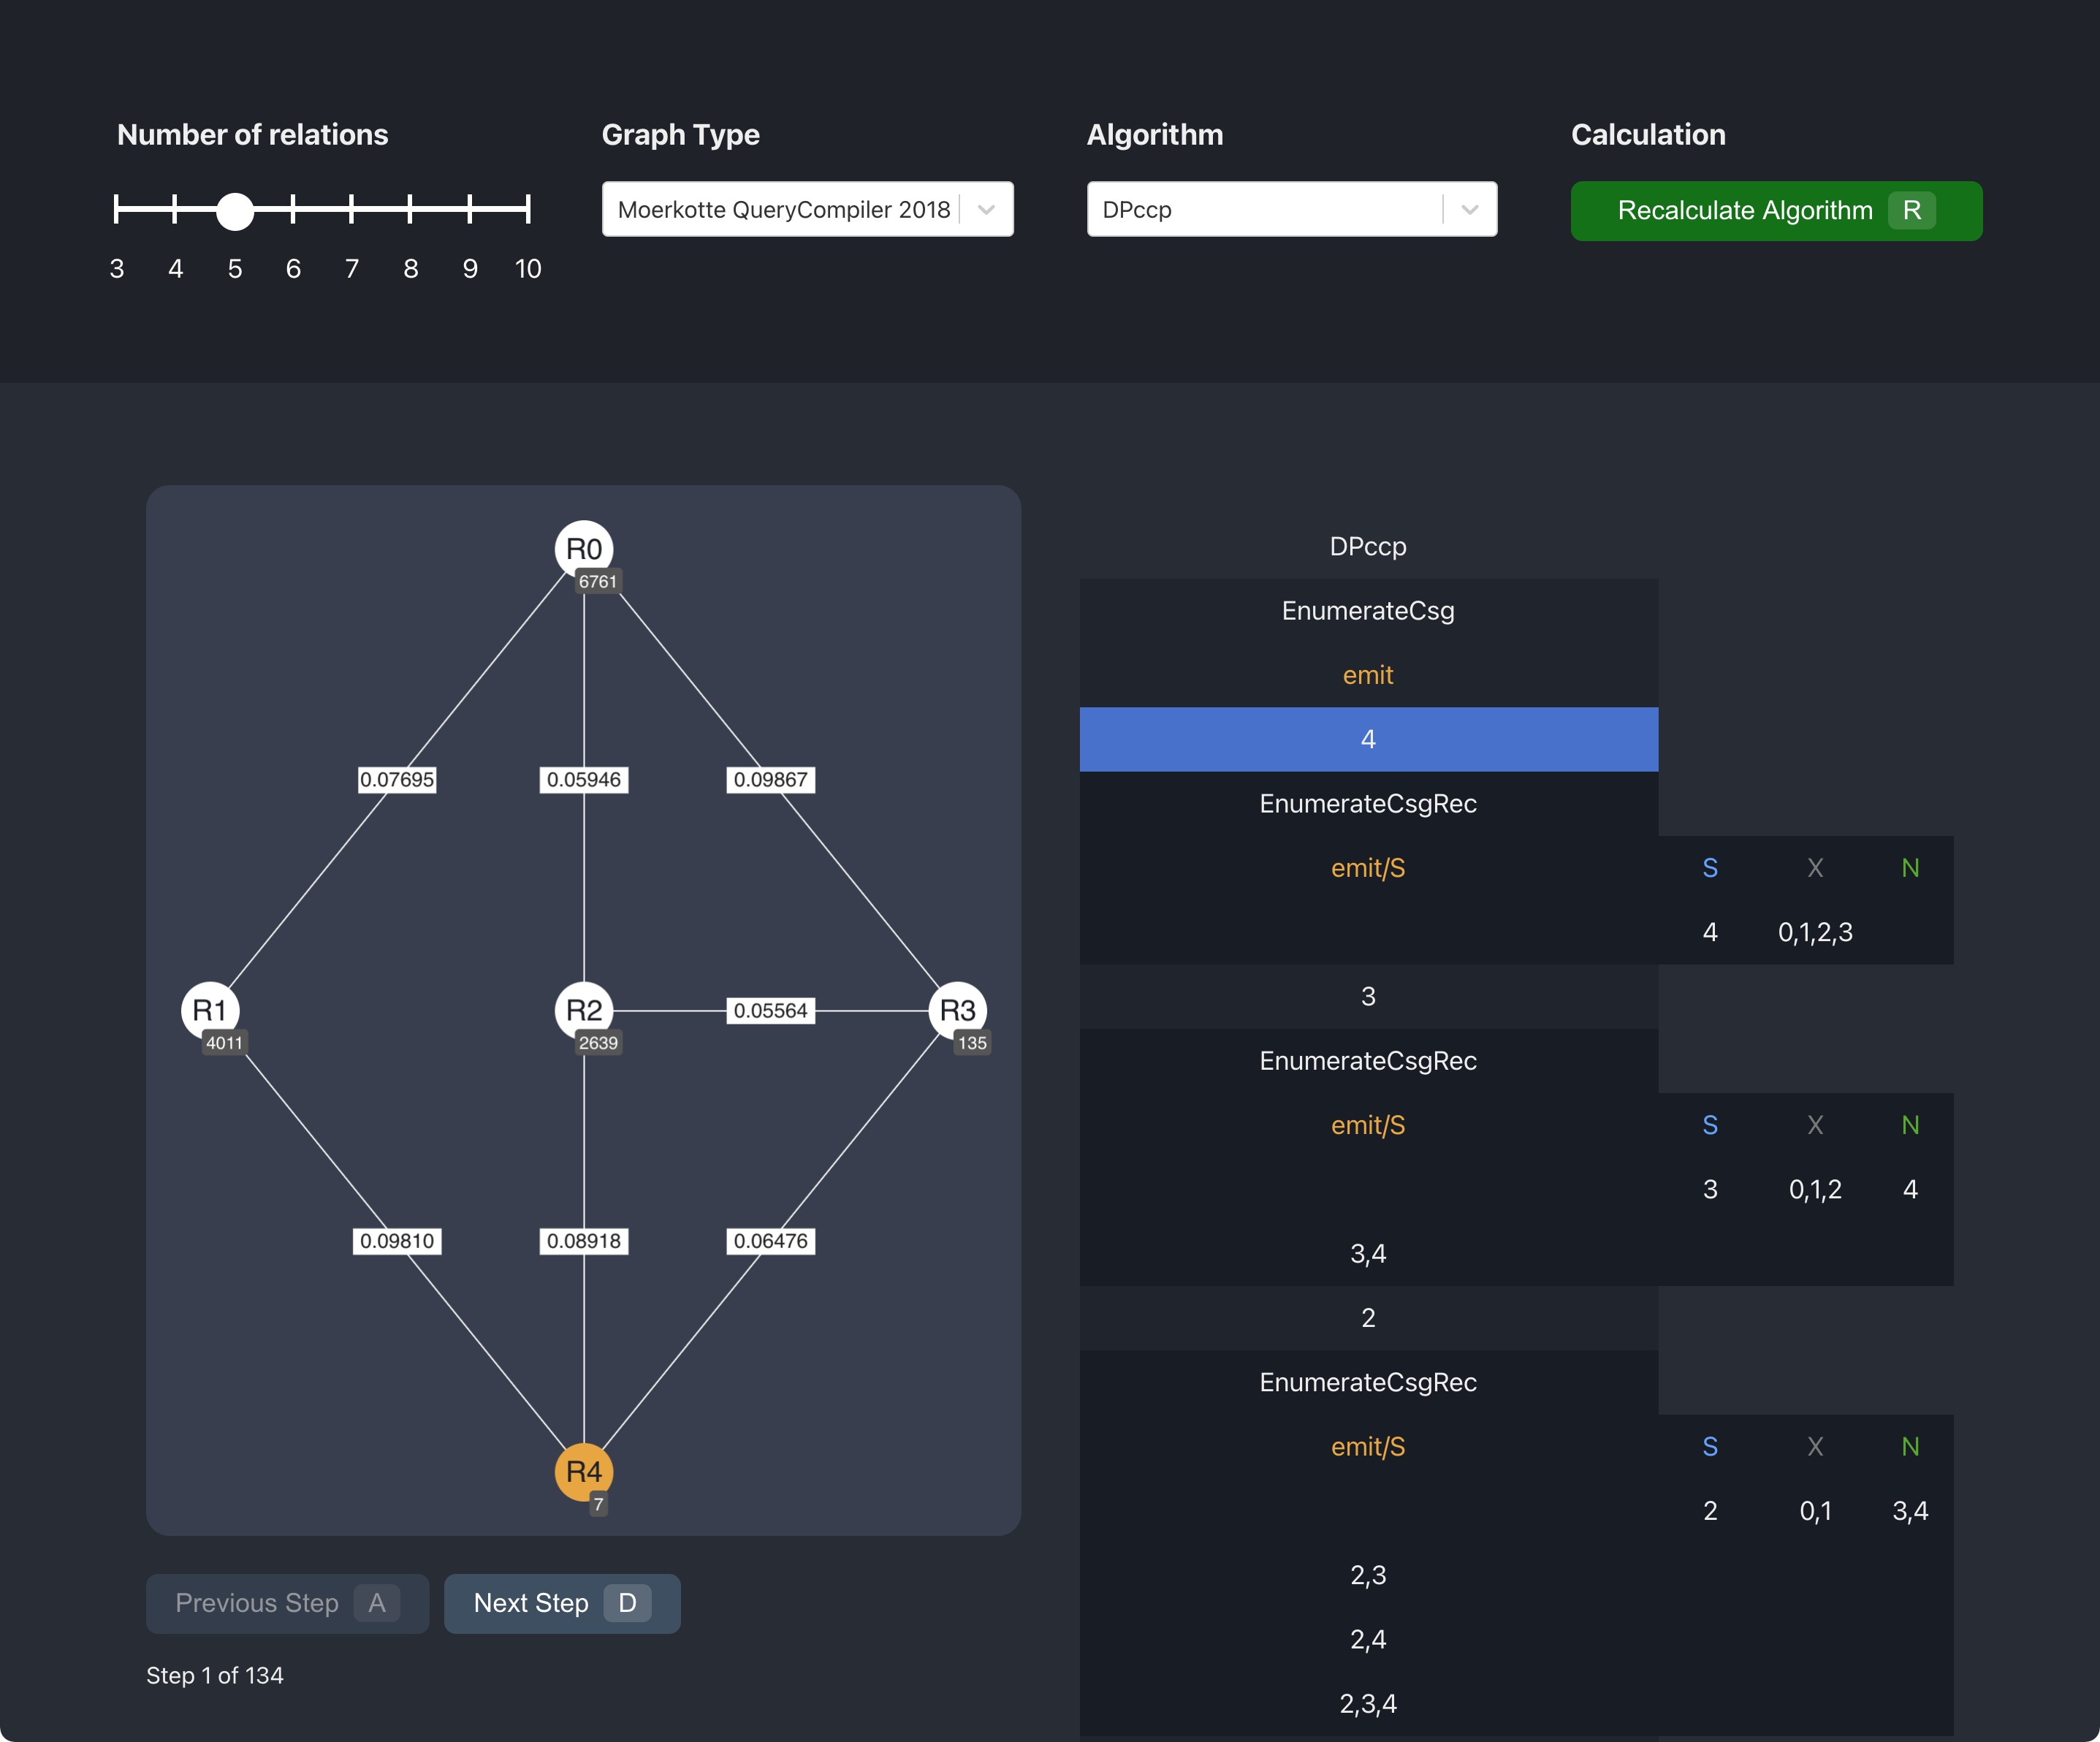
\includegraphics[width=\textwidth + 2cm]{img/renderedVisualization.png}
    \caption[Sample rendered result of \texttt{DPccp} on a ``Moerkotte 2018'' query graph at step 1]{Sample rendered result of \texttt{DPccp} on a ``Moerkotte 2018'' query graph at step 1. The variable table on the right is scrollable to reveal more steps.}
    \label{fig:sample-rendered-dpccp}
\end{figure}

\subsubsection{Building}
As the project makes heavy use of the ECMAScript 2020\footnote{\url{https://www.ecma-international.org/publications/standards/Ecma-262.htm}} syntax, it is transpiled using the Babel\footnote{\url{https://babeljs.io}} cross-compiler to a more downwards-compatible JavaScript version when building the project to improve browser support.

\paragraph{Linting}
For the client-side code we use ESLint\footnote{\url{https://eslint.org}} configured with the \texttt{"react-app"} template\footnote{\url{https://github.com/facebook/create-react-app/blob/master/.eslintrc.json}}, which itself is an extension of the \texttt{"eslint:recommended"} template as specified on \url{https://eslint.org/docs/rules/}.

\paragraph{Dependencies}

Since we're restructurig the files from the QueryCompiler exercise to increase modularity and reusability . We define all packages in a way that no cyclical dependencies exist.

\subsection{Installation and Development}

\subsubsection{Prerequisites}
\label{subsub:implementation-prerequisites}

In order to run the project locally some prerequisites have to be fulfilled:
\begin{itemize}
    \item A state-of-the-art web browser has to be installed, such as a recent version of Google Chrome\footnote{\url{https://www.google.com/chrome/}}, Mozilla Firefox\footnote{\url{https://www.mozilla.org/firefox/}}, Microsoft Edge\footnote{\url{https://www.microsoft.com/edge}}, or Apple Safari\footnote{\url{https://www.apple.com/safari/}}
    \item The Go programming language has to be installed according to the official installation guidelines\footnote{\url{https://golang.org/doc/install}}
    \item The Go environment has to be set up, namely correctly specifying the \texttt{\$GOOROOT} and \texttt{\$GOPATH} environment variables. Furthermore, the project has to be moved to the \texttt{\$GOPATH/src} directory
    \item The Node Package Manager (npm) has to be installed along with the Node.js runtime\footnote{\url{https://www.npmjs.com/get-npm}}
    \item While not required, it is strongly recommended to install the Git\footnote{\url{https://git-scm.com}} distributed version control system 
\end{itemize}

\subsubsection{Dependencies}
\label{subsub:dependencies}

\paragraph{Client}
Client dependencies are maintained in the \texttt{package.json} file of the project's \texttt{client} directory. All client repositories have to be installed by navigating to the \texttt{client} directory and then using the following command:
\begin{minted}{shell-session}
$ npm install
\end{minted}

\paragraph{Server}
The server-side code dependencies are defined in the \texttt{go.mod} file of the project's \texttt{server} directory. They can be installed by navigating to the \texttt{server} directory and then using the following command:
\begin{minted}{shell-session}
$ go get ./...
\end{minted}

\subsubsection{Local Development}
Once dependencies are installed as specified in section \ref{subsub:dependencies}, the project can be run locally by navigating to the project directory in a Unix shell (macOS and Linux) or PowerShell (Windows) and running

\begin{minted}{shell-session}
    $ cd server && go run main.go
\end{minted}
and, in another shell instance,
\begin{minted}{shell-session}
    $ cd client && npm start
\end{minted}

This will start two locally running web servers that can be accessed via \url{https://localhost:8080/} (Server) and \url{https://localhost:3000/} (Client).

\begin{note}
As the client is fetching its data from the server please keep in mind that the server has to be started \textit{before} accessing the client URL.
\end{note}

\subsection{Deployment}
One of the major benefits of using a client-server architecture and web technologies is that we can host the server part on an application server or platform-as-a-service offering such as Google's Cloud App Engine\footnote{\url{https://cloud.google.com/appengine}} and the front-end (client) on a web server.
This way, the user of the visualization neither has to install nor update the application himself, as this duty is completely on the host's side. Likewise, the deployment of new application versions is simple and can be done with a single shell instruction for both client and server.

In the following we demonstrate how to set up the entire application stack, both client and server, in order to get from the cloned repository to a deployed application using the Google Cloud SDK\footnote{\url{https://cloud.google.com/sdk}} for the server-side application and GitHub Pages\footnote{\url{https://pages.github.com}} for hosting the front-end.

\paragraph{Prerequisites}   

\subparagraph{Server}
The Google Cloud SDK must be installed using 
\begin{minted}{shell-session}
    $ curl https://sdk.cloud.google.com | bash
\end{minted}
Follow the instructions in the terminal session to continue. 

\subparagraph{Client}
All Node.js 